\documentclass{standalone}
\usepackage{tikz}
\begin{document}
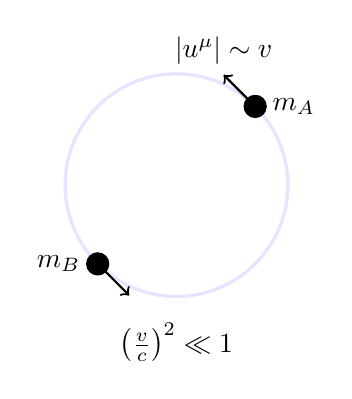
\begin{tikzpicture}
    %\node[] at (0,1.7) {\small{$\delta h_{+,\times}(t)\approx A_{GR}(t) \exp\left(i\delta\Psi_{vis} t\right)$}};
    \filldraw[color=blue!10, fill=white, very thick](0,0) circle (1.414);
    %\draw[thick    ] ( 0, 0) -- node[above left] {\small{$r$}} ++ (1,1);
    \filldraw[black] ( 1, 1) circle (4pt) node[right] { $\;m_A$};
    \draw[thick, ->] ( 1, 1) -- ( 0.6, 1.4) node[above] {$|u^{\mu}|\sim v$};
    \filldraw[black] (-1,-1) circle (4pt) node[left] { $m_B\;$};
    \draw[thick, ->] (-1,-1) -- (-0.6,-1.4) ;
    \node[] at (0,-2) {$\left(\frac{v}{c}\right)^2 \ll 1$};
    \end{tikzpicture}
\end{document}

